\documentclass{article}

\usepackage[utf8]{inputenc}
\usepackage{setspace}
\usepackage{geometry}
\usepackage{graphicx}
\usepackage{caption}
\usepackage{indentfirst}
\usepackage{anyfontsize}
\usepackage{textcomp}
\usepackage{amsmath}
\usepackage{float}
\usepackage{changepage}
\usepackage [english]{babel}
\usepackage [autostyle, english = american]{csquotes}
\MakeOuterQuote{"}

\graphicspath{}



\title{Lotka Volterra Modeling}
\author{Geneva Porter}
\date{23 October 2018}

%\begin{figure}[H]
%\centering{\includegraphics[width=10cm]{FILENAME.eps}}
%	\caption{CAPTION}
%\end{figure}

%$\begin{bmatrix}
%11      & 12  \\
%21      & 22  \\
%\end{bmatrix}$

\begin{document}
	
\begin{titlepage}
\maketitle
\thispagestyle{empty}


\begin{center}
	
\large \it San Diego State University 
	
Professor J Mahaffy, Math 636

\end{center}
\end{titlepage}

\section*{Introduction}

The widespread application of DDT to control insects in the later 20th century has led to serious and long-lasting environmental problems. The agricultural industry was a significant contributor to many such problems by using DDT to control the population of scale insects. Although DDT was an extremely effective pesticide, it was not perfect. Some insects survived, and when they reproduced, their offspring were more likely to inherit that resistance. Now there were fewer insects to compete with, an abundant food supply, and an ineffective pesticide: a perfect recipe for rapid multiplicity. Naturally, this made insect control even more difficult. It left farmers with two options: to increase the use of DDT, or find an alternate pesticide. No other pesticide came close to the effectiveness of DDT at the time, so even more was used. By poisoning the insects, a fundamental component of the food chain, larger animals began to suffer. The insects they were eating and feeding to their young were slowly poisoning the animal population at several levels. Rachel Carson highlighted this in her 1962 book {\it Silent Spring}, detailing the devastation of the bird population as a direct result of the excessive use of DDT.

The DDT explosion seemed like a godsend at the beginning: crops were flourishing, malaria was nearly eradicated, and chemical manufacturing companies saw great success. Of course, it was not long before the devastating side effects began to show. For frmers, DDT became like agricultural heroin; the rising demand only provided a temporary high to a dying farm. Of course, farmers found that they needed more and more DDT to keep crops free of insects that had adapted with DDT resistance. The more the farmers demanded, the more the chemical companies made. The large-scale purchase of DDT became a significant financial burden to farmers, driving them into debt. Farmers also lost money when crops themselves were poisoned with DDT. The cranberry industry took a significant loss when DDT was applied during the wrong growth cycle stage, resulting in the recall of cranberry products across the nation.

Today we have smarter methods of controlling pests. Using population modeling, we can guide species to a favorable equilibrium by continually introducing natural predators into the habitat. For example, ladybugs are now prevalent as pest controllers, as they eat aphids and other scale insects. If we adjusted the parameters for a predator-prey model, we could gain a good idea of how many ladybug immigrants are needed to sustain an equilibrium with lower numbers of pests.   

\section*{Model Types}

Here we will be using Lotka-Volterra models to investigate population dynamics between hare and Lynx. The Lotka-Volterra model variation we will examine first is given by:

\vspace{3mm}

\hspace{5mm}	$\dot{H}=a_1H-a_2HL-a_3H^2$

\vspace{3mm}

\hspace{5mm}	$\dot{L}=-b_1L+b_2HL$

\vspace{3mm}


This model includes an additional parameter, $-a_3$, that accounts for the crowding effect of the hares when the lynx population is low. This term ensures that the hare population will not grow unbounded with the absence of a lynx population. We can analyze the stability of this model by first setting each equation to zero and solving for $(H,L)$. This gives us:

\vspace{3mm}

\hspace{5mm} $e_1:(0,0)$ \hspace{5mm} $e_2:(\dfrac{a_1}{a_3},0)$ \hspace{5mm} $e_3:(\dfrac{b_1}{b_2}, \dfrac{a_1b_2-a_3b_1}{b_2a_2})$

\vspace{3mm}

Note that $a_1b_2-a_3b_1>0$ for our population equilibria to be strictly positive. Next, our Jacobian matrix and eigenvalues give us conditions for the stability of our fixed points:

\vspace{3mm}

\hspace{5mm}$\begin{bmatrix}
\partial\dot{H}/\partial H      & \partial\dot{H}/\partial L  \\
\partial\dot{L}/\partial H      & \partial\dot{L}/\partial L  \\
\end{bmatrix}=$
$\begin{bmatrix}$
$a_1-a_2L-2a_3H      & -a_2H  \\
b_2L      & -b_1+b_2H  \\
\end{bmatrix}$

\vspace{3mm}

\hspace{5mm}$\lambda_{e1,1}=a_1$ and $\lambda_{e1,2}=-b_1$

\vspace{3mm}

\hspace{5mm}$\lambda_{e2,1}=-a_1$ and $\lambda_{e2,2}=\dfrac{a_1b_2-a_3b_1}{a_3}$

\vspace{3mm}

\hspace{5mm}$\lambda_{e3}$: $\lambda^2+\lambda(\dfrac{a_3b_1}{b_2})+(\dfrac{b_1}{b_2})(a_1b_2-a_3b_1)=0$

\vspace{3mm}

We assume all parameters for this model are positive, so both $e_1$ and $e_2$ are unstable saddles. If we examine the characteristic equation for $e_3$, our solutions for $\lambda$ must both have negative real components, so the equilibrium is stable. If $a_3(a_3b_1)/(4b_2)<a_1b_2-a_3b_1$, then we will have an asymptotically stable node. Otherwise we will have complex eigenvalues and a stable spiral. In either case, all equilibria are structurally stable.

\vspace{3mm}

Another variation of the Lotka-Volterra model includes a Holling's Type II term, given by:

\vspace{3mm}

\hspace{5mm}	$\dot{H}=a_1H-\dfrac{a_2HL}{1+k_1H}$

\vspace{3mm}

\hspace{5mm}	$\dot{L}=-b_1L+\dfrac{b_2HL}{1+k_1H}$

\vspace{3mm}


 This modified term accounts for the possibility that the hare population could satiate the lynx. Notice that if the $k_1$ term is very small, the model is essentially the linear portions of part (a). Again, we can analyze the stability of this model. This gives us:
 
 \vspace{3mm}
 
 \hspace{5mm}$e_1:(0,0)$ \hspace{5mm} $e_2:(\dfrac{b_1}{b_2-b_1k_1}, \dfrac{a_1b_2}{a_2(b_2-b_1k_1)})$
 
 \vspace{3mm} 
 
 Note that $b_2-b_1k_1>0$ for our population equilibria to be strictly positive. Next, our Jacobian matrix and eigenvalues give us conditions for the stability of our fixed points:
 
 \vspace{3mm}

\hspace{5mm}$\begin{bmatrix}
\partial\dot{H}/\partial H      & \partial\dot{H}/\partial L  \\
\partial\dot{L}/\partial H      & \partial\dot{L}/\partial L  \\
\end{bmatrix}=
\begin{bmatrix}
a_1-a_2L/(1+k_1H)^2      & -a_2H/(1+k_1H)  \\
b_2L/(1+k_1H)^2      & -b_1+b_2H/(1+k_1H)  \\
\end{bmatrix}$

 \vspace{3mm}

\hspace{5mm}$\lambda_{e1,1}=a_1$ and $\lambda_{e1,2}=-b_1$

 \vspace{3mm}

\hspace{5mm}$\lambda_{e2}$: $\lambda^2-\lambda(\dfrac{a_1b_1k_1}{b_2})+\dfrac{a_1b_1}{b_2}(b_2-b_1k_1)=0$

 \vspace{3mm}
 
 Since all parameters for this model are positive, we can see that $e_1$ and is a saddle node and thus unstable. If we examine the characteristic equation for $e_2$, we can see that our solutions for $\lambda$ must have positive real components, so the equilibrium is unstable. If $(k_1^2)/(4b_2)>b_2-b_1k_1$, then we will have real eigenvalues and an unstable node. If the inequality sign is reversed, we will have complex eigenvalues and an unstable spiral. Both equilibria are structurally stable.

\section*{Hare and Lynx Dynamics}

We will be using the previous variations of the Lotka-Volterra model to investigate species of hare and lynx. We will examine data from 1900 to 1930 regarding the population of hares and lynx (as given by the number of pelts taken) provided by the Hudson's Bay Company in Canada. Our first investigation will be a linear analysis model. This model is given by:

 \vspace{3mm}

\hspace{5mm}$\dot{H}=a_1H-a_2HL$

\vspace{3mm}

\hspace{5mm}$\dot{L}=-b_1L+b_2HL$

 \vspace{3mm}

We begin by looking at only the first 20 years of data. The following parameters were found using Matlab to minimize the sum of square errors:

 \vspace{3mm}

\hspace{5mm}$H(0)=34.9134$, $L(0)=3.8566$, $a_1=0.48069$, $a_2=0.024822$, $b_1=0.92718$, $b_2=0.027564$

 \vspace{3mm}
 
 The equilibria for the presence of both species was found, as well as the sum of squared errors:
 
  \vspace{3mm} 

\hspace{5mm} $e=(33.637,19.365)$, SSE = 594.94
 
  \vspace{3mm}
  
  Figures 1 and 2 show the time series representation of the species and the phase portrait with equilibrium, respectively.

 \vspace{3mm}
 
  Next, we examined the population over all 30 years. The parameters, equilibria, and sum of squared errors were found:
 
 \vspace{3mm}
 
 \hspace{5mm}$H(0)=28.4037$, $L(0)=8.2310$, $a_1=0.68130$, $a_2=0.028570$, $b_1=0.62262$, $b_2=0.021734$
 
 \vspace{3mm} 
 
 \hspace{5mm}$e=(28.648,23.846)$, SSE = 4564.36
 
 \vspace{3mm}
 
 Figures 3 and 4 show the time series representation of the species and the phase portrait with equilibrium, respectively.
 
 \vspace{3mm}
 
 Looking at both models, we can see several differences. The 20 year model better fits the data, which we can see by noticing that the peaks are closer to the maximum for each period. This is apparent in both species, but particularly for the hare population. This is expected, as the data for the hare population is very low from 1925-1930, which weighted the curve toward a smaller amplitude. The sum of square errors for the 20 year model is also significantly lower, even considering the added data points in the 30 year model. The phase portrait for the 30 year model has a tighter orbit as the amplitude of the time series curves are lower. Also, the dual-species equilibrium is closer to the identity line in the 30 year model. In this sense the 20 year model is a bit more realistic, as it seems there should be a more significant difference in hare and lynx population at the equilibria. Surely, there needs to be a much higher hare population to sustain a significant lynx population. It is understandable that a smaller time frame would yield a more accurate model, as there is simply less data to weigh.
 
 \vspace{3mm}

\begin{figure}[H]
\centering{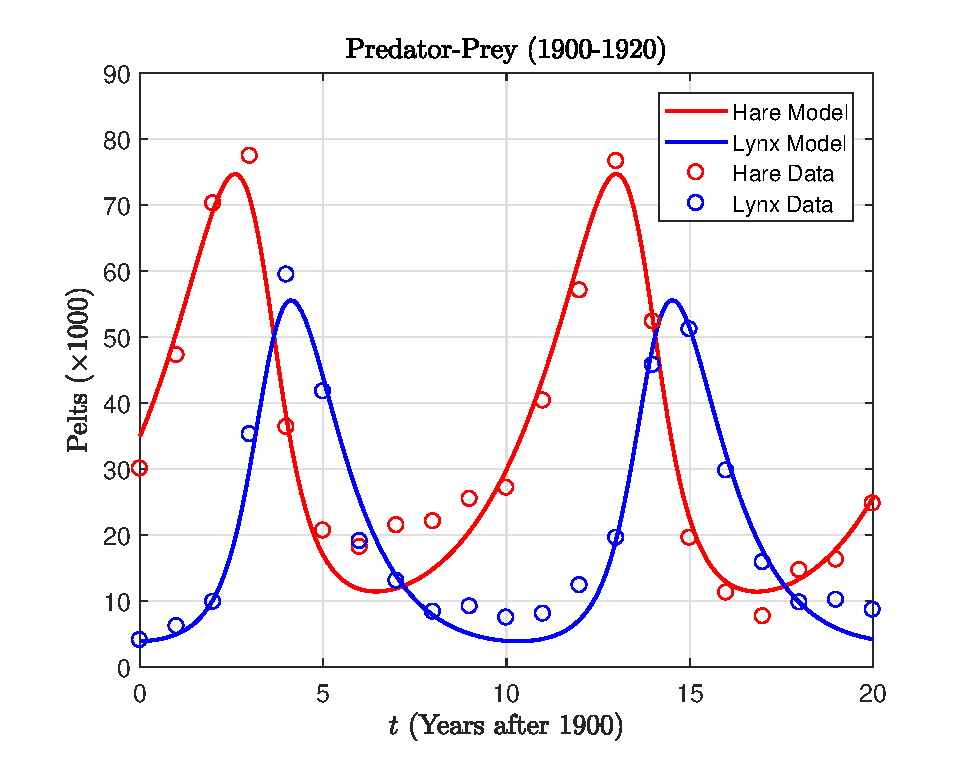
\includegraphics[width=11cm]{LV01.eps}}
	\caption*{\textbf{Figure 1}}
\end{figure}


\begin{figure}[H]
	\centering{\includegraphics[width=11cm]{LV02.eps}}
	\caption*{\textbf{Figure 2}}
\end{figure}


\begin{figure}[H]
	\centering{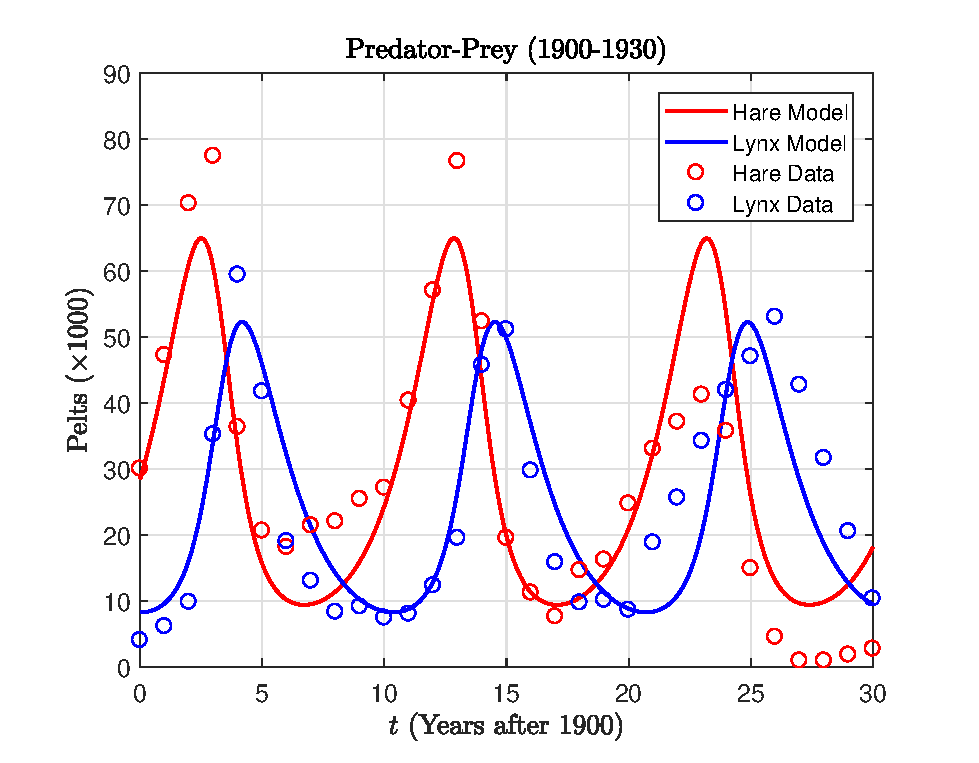
\includegraphics[width=11cm]{LV03.eps}}
	\caption*{\textbf{Figure 3}}
\end{figure}

\begin{figure}[H]
	\centering{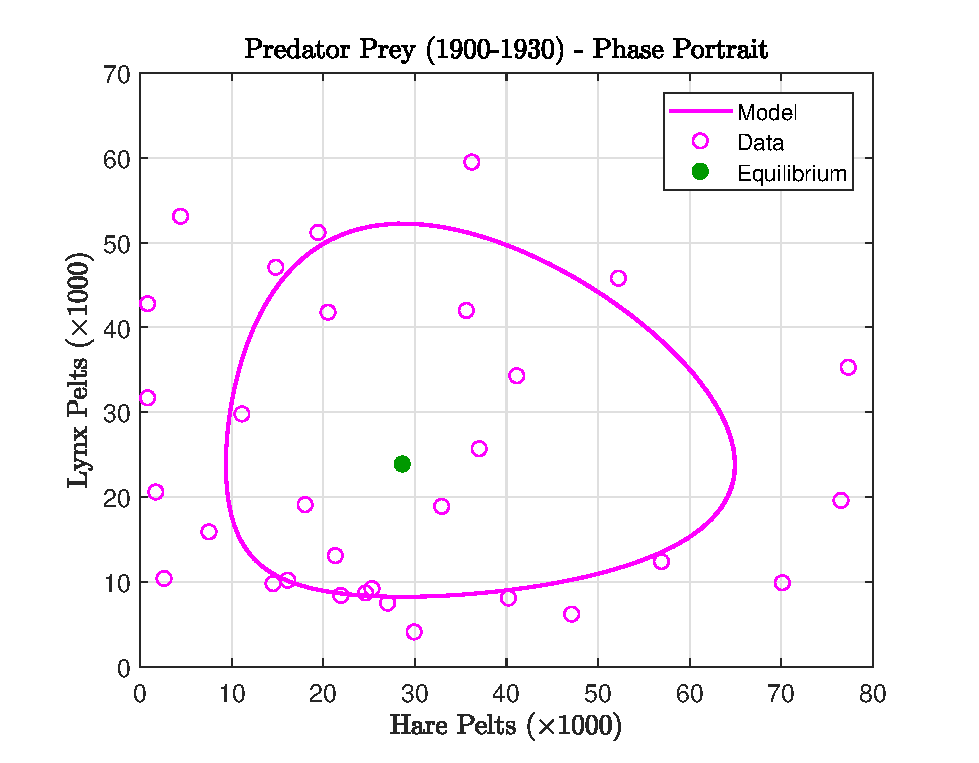
\includegraphics[width=11cm]{LV04.eps}}
	\caption*{\textbf{Figure 4}}
\end{figure}

Now we will add the carrying capacity term back onto our linear model, giving us:

\vspace{3mm} 

\hspace{5mm}$\dot{H}=a_1H-a_2HL-a_3H^2$

\vspace{3mm} 

\hspace{5mm}$\dot{L}=-b_1L+b_2HL$

\vspace{3mm} 

For this model, the following parameters, dual-species equilibria, and sum of squared errors were found:

\vspace{3mm} 

\hspace{5mm}$H(0)=28.1361$, $L(0)=5.7224$

\vspace{3mm}

\hspace{5mm}$a_1=0.72781$, $a_20.029019$, $a_3=0.0011380$, $b_1=0.61862$, $b_2=0.022299$

\vspace{3mm} 

\hspace{5mm}$e=(27.742,23.993)$, SSE = 4237.97

\vspace{3mm} 

Figures 5 and 6 show the time series representation of the species and the phase portrait with the equilibrium, respectively.

\begin{figure}[H]
	\centering{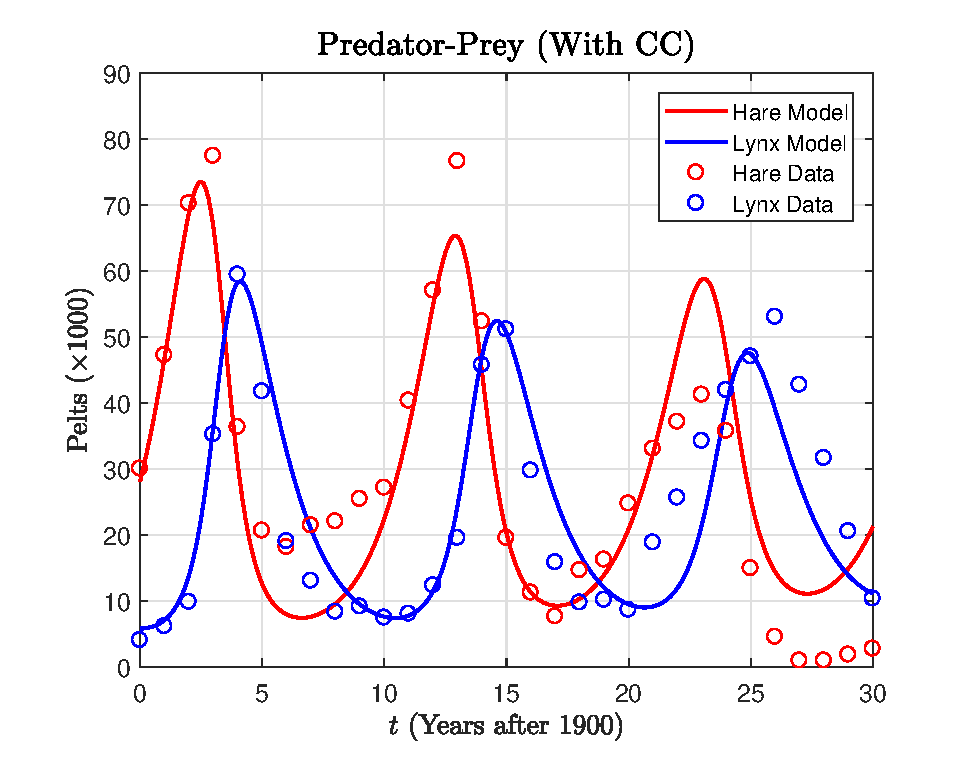
\includegraphics[width=11cm]{LV05.eps}}
	\caption*{\textbf{Figure 5}}
\end{figure}

\begin{figure}[H]
	\centering{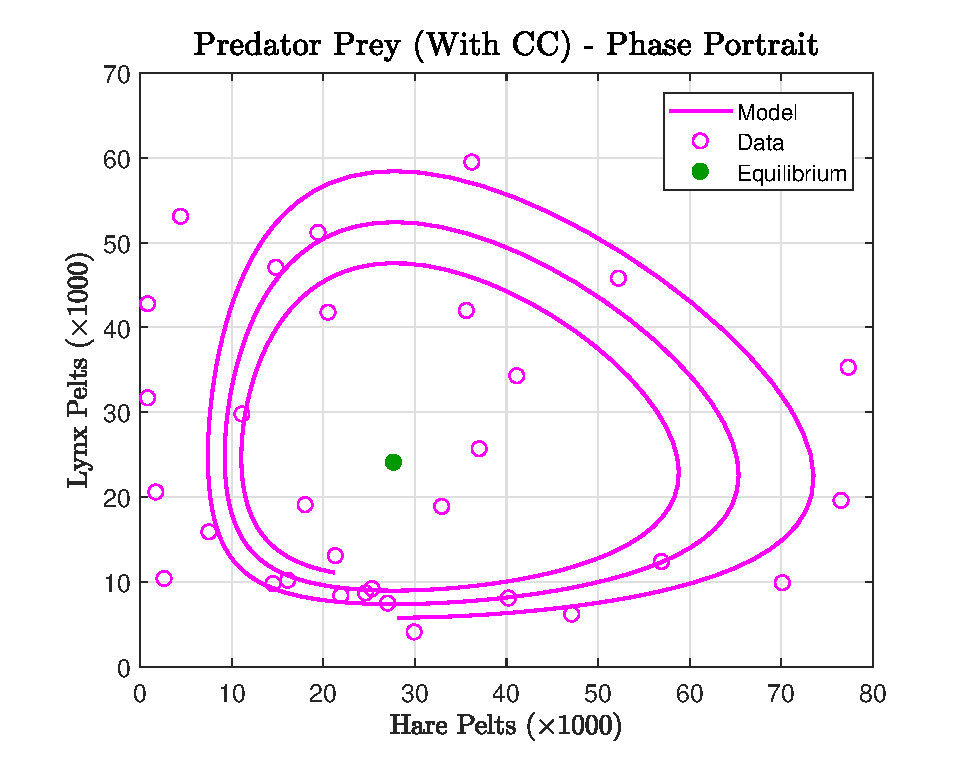
\includegraphics[width=11cm]{LV06.eps}}
	\caption*{\textbf{Figure 6}}
\end{figure}

\vspace{3mm}

For our stability analysis, we will use the generic results from above to calculate the eigenvalues for all 3 equilibria:

\vspace{3mm}

\hspace{5mm}$e_1=(0,0)$, $\lambda_{e1,1}=0.72781$ and $\lambda_{e1,2}=-0.61862$

\vspace{3mm}

\hspace{5mm}$e_2=(639.563,0)$, $\lambda_{e2,1}=-0.72781$ and $\lambda_{e2,2}=13.6431$

\vspace{3mm}

\hspace{5mm}$e_3=(27.742,23.993)$, $\lambda_{e3}=-0.015785\pm0.65609i$

\vspace{3mm}

 All 3 equilibria are structurally stable. We can see that our total extinction equilibria and lynx extinction equilibria are saddle nodes. The extinction equilibria is shown in Figure 7 at (0, 0). The lynx extinction equilibria is not shown, as it would compromise the readability of the graph were it to be included. The dual-species equilibrium has complex eigenvalues with negative real components, so it is a stable spiral point. This is also illustrated in the phase portrait, where we can see the orbit sinking into the equilibrium of (27.742, 23.993). This indicates that the model predicts a constant population of hare and lynx in the future, with each population curve in the time series oscillating and dampening about the lines $P=27.742$ for hares and $P=22.993$ for lynx. This prediction is not reasonable. One reason is that the likelihood of the birth and death rate being equal would be improbable. Constant populations are unheard of: changing food availability, mating seasons, and weather patterns are just some of the factors that influence changing populations over the course of even a single year. However, with the small window we are looking at, the model fits the data well. The data shows a dampening happening each period, and the model reflects that well (even though such dampening could not continue long term). This effect is not seen in the linear model, which may be more realistic long-term.


\begin{figure}[H]
	\centering{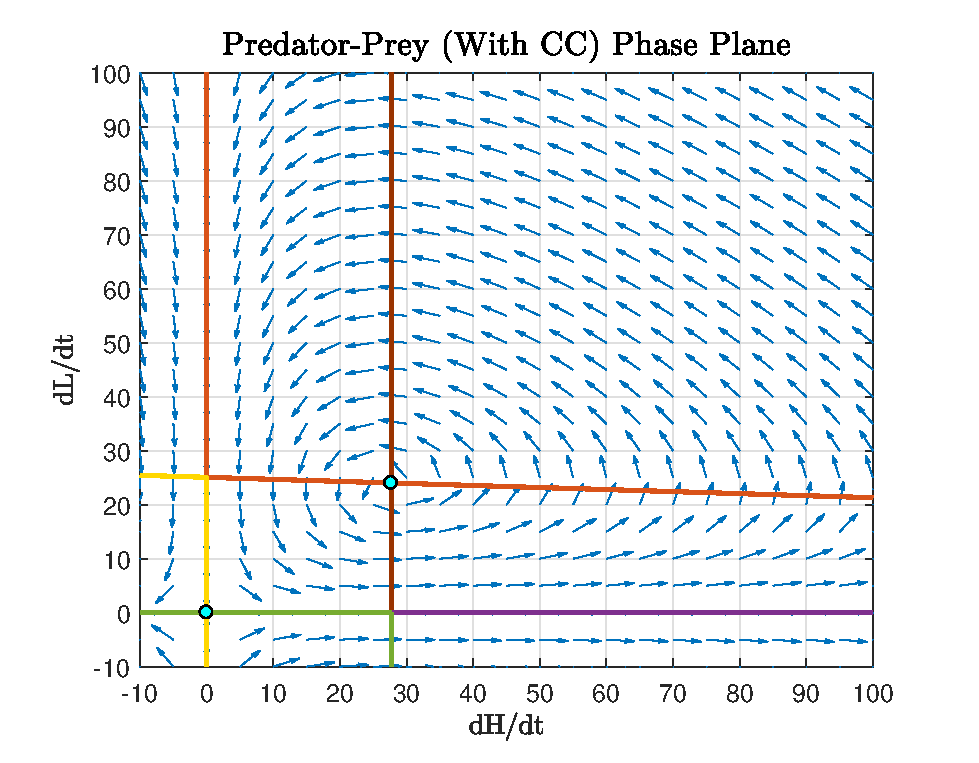
\includegraphics[width=11cm]{LV07.eps}}
	\caption*{\textbf{Figure 7}}
\end{figure}

Now we will consider the model with the Holling's Type II parameter, given by:

\vspace{3mm}

\hspace{5mm}	$\dot{H}=a_1H-\dfrac{a_2HL}{1+k_1H}$

\vspace{3mm}

\hspace{5mm}	$\dot{L}=-b_1L+\dfrac{b_2HL}{1+k_1H}$

\vspace{3mm}

For this model, the following parameters, dual-species equilibria, and sum of squared errors were found:

\vspace{3mm} 

\hspace{5mm}$H(0)=28.4219$, $L(0)=8.2287$

\vspace{3mm}

\hspace{5mm}$a_1=0.68181$, $a_2=0.028592$, $b_1=0.62207$, $b_2=0.021722$, $k1=9.2586\cdot10^{-14}$

\vspace{3mm} 

\hspace{5mm}$e=(28.64,23.85)$, SSE = 4564.52

\vspace{3mm} 

Figures 8 and 9 show the time series representation of the species and the phase portrait with the equilibrium, respectively. 

\begin{figure}[H]
	\centering{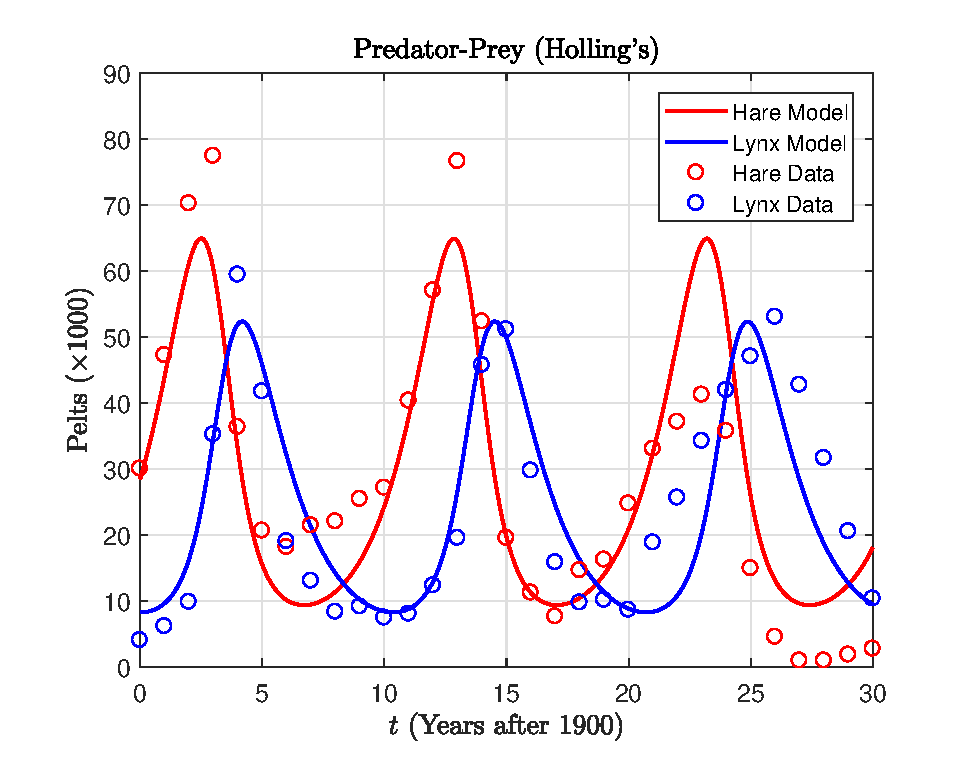
\includegraphics[width=11cm]{LV08.eps}}
	\caption*{\textbf{Figure 8}}
\end{figure}

\begin{figure}[H]
	\centering{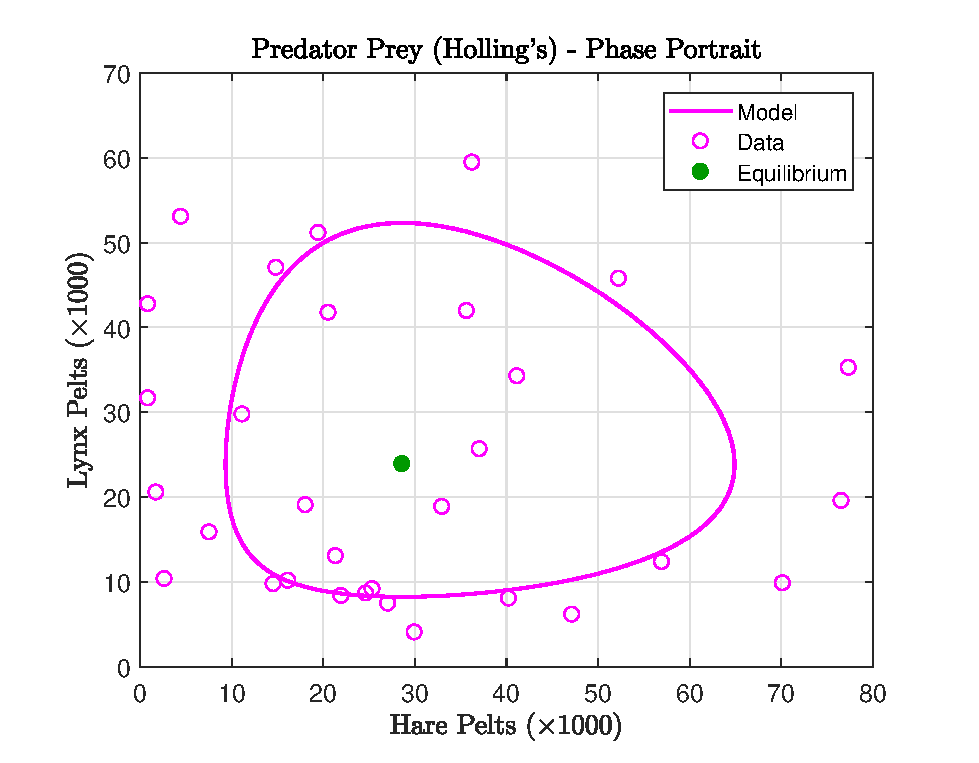
\includegraphics[width=11cm]{LV09.eps}}
	\caption*{\textbf{Figure 9}}
\end{figure}

For our stability analysis, we will use the generic results from the Holling's Type II term analysis to calculate the eigenvalues for both equilibria:

\vspace{3mm} 

\hspace{5mm}$e_1=(0,0)$, $\lambda_{e1,1}=0.68181$ and $\lambda_{e1,2}=-0.62207$

\vspace{3mm} 

\hspace{5mm}$e_2=(28.637,23.846)$, $\lambda_{e2}=9.0388\cdot10^{-13}\pm0.65126i$

\vspace{3mm} 

Here, both equilibria are unstable. The total extinction equilibrium is a saddle node and the dual-species equilibria is an unstable spiral. Because the spiral is growing very gradually, the shape is not visible on the phase portrait graph. We can also see this by examining the real component of the eigenvalues. It is very small, indicating that the change of population growth is happening slowly. This unstable spiral predicts that the time series population curves will increase in amplitude, resulting in higher maximums and lower minimums. This behavior may be reasonable, but will eventually result in negative populations. It is also a less effective fit, as the data indicates a dampening in altitude over time rather than an increase in altitude.

\begin{figure}[H]
	\centering{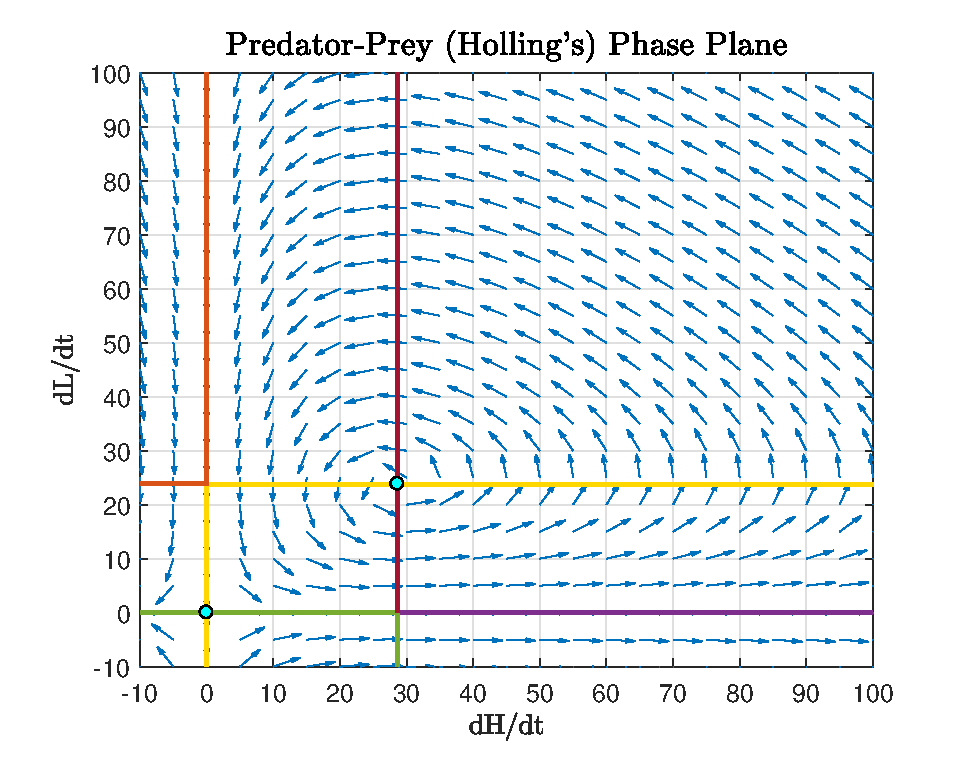
\includegraphics[width=10cm]{LV10.eps}}
	\caption*{\textbf{Figure 10}}
\end{figure}

\section*{Conclusion}

The linear model, carrying capacity model, and Holling's Type II model each have strengths and weaknesses. Over a long time period, the linear model seems most reasonable. The amplitude is constant, so the model can predict realistic behavior over a long time given that the period length for the data remains roughly constant. In the short term, the carrying capacity model is the most effective. It accounts for the dampening amplitude and the availability of food for hares. The Holling's Type II model seems the least effective; even though is closely resembles the linear model, its long term behavior is not reasonable.

\end{document}





































